\documentclass{beamer}
\usepackage[utf8x]{inputenc}
\usepackage[ngerman]{babel}
\usepackage{amsmath}
\usepackage{amsfonts}
\usepackage{amssymb}
\usepackage{graphicx}
\usepackage{subfigure}
\author{Johannes Hackel und Falco Prescher}
\title{Testgetriebene Entwicklung}

\usetheme{Ilmenau}
\useoutertheme{split}
\usecolortheme{rose}

\begin{document}

\begin{frame}
\titlepage
\end{frame}

\begin{frame}
\frametitle{Gliederung}
\tableofcontents
\end{frame}

\section{Allgemeines zur testgetriebenen Entwicklung}
\begin{frame}
\frametitle{Allgemeines zur testgetriebenen Entwicklung}
\end{frame}

\section{Vorgehensweise der testgetriebenen Entwicklung}
\begin{frame}
\frametitle{Entwicklungszyklus}
\begin{figure}[htbp]
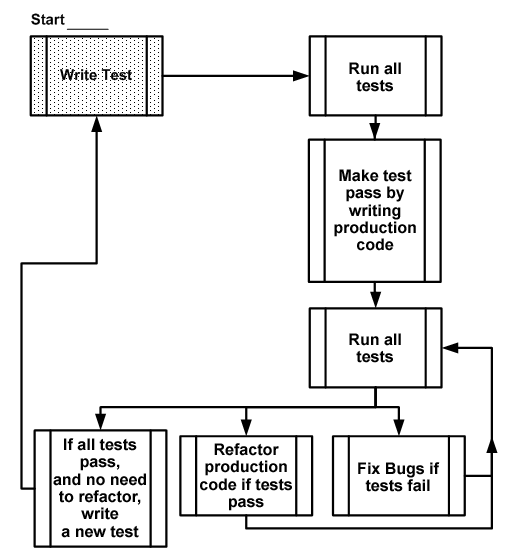
\includegraphics[width=5cm]{zyklus.png}
\caption{Der Entwicklungszyklus von Software mittels testgetriebener Entwicklung}
\end{figure}
\end{frame}

\section{Das Inversion Of Control im Zusammenhang mit Mocks}
\begin{frame}
\frametitle{Stubs}
\begin{itemize}
\item Stub - engl. für Platzhalter
\item Steuerbarer Ersatz für eine existierende Abhängigkeit
\item Ermöglicht testen des Coes ohne sich direkt mit der Abhängigkeit auseinanderzusetzen
\end{itemize}
\end{frame}


\begin{frame}
\frametitle{Mocks}
\begin{itemize}
\item Mocking - engl. für Vortäuschen
\item Erstellung eines Versuchsobjektes durch eine vorgetäuschte Implementierung von Schnittstellen oder abstrakten Klassen
\item Erzeugung des Objektes während der Laufzeit durch Mockframeworks
\item Enthalten Konfigurations- und Testverifizierungsmöglichkeiten für Unit Tests (Erwartungsgemäße Interaktionen des Mockobjektes wird getestet)
\item Mockframeworks: Mockito\footnote{http://www.code.google.com/p/mockito/} (Java) und Moq\footnote{http://www.code.google.com/p/moq/} (.NET)
\end{itemize}
\end{frame}

\begin{frame}
\frametitle{Inversion Of Control}
\begin{itemize}
\item kurz IoC - engl. für Steuerungsunkehrung
\item Aufrufen von benutzerspezifische Methoden durch das Verhalten eines Softwareframeworks
\item Dependency Injection (DI) = Spezialform des IoC\\Möglichkeit zur Registrierung Schlüssel-Wertpaaren zu einem IoC-Container in einer Startsequenz (Bootstrap)
\item Schlüssel = abstrakte Klasse oder Schnittstelle\\Wert = Methode zur Rückgabe eines Objektes (Bsp. Konstruktoren oder Methoden)
\item Inversion Of Control - Frameworks:
PicoContainer\footnote{http://www.picocontainer.codehaus.org/} (Java) und StructureMap\footnote{http://www.docs.structuremap.net/} (.NET)
\end{itemize}
\end{frame}

\begin{frame}
\frametitle{Inversion Of Control}
\begin{figure}[htbp]
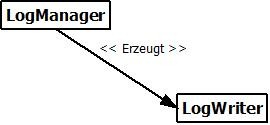
\includegraphics[width=7cm]{logging_closeCoupled.jpg}
\caption{LogManager ist direkt abhängig von einer konkreten Implementierung von LogWriter}
\end{figure}
\end{frame}

\begin{frame}
\frametitle{Inversion Of Control}
\begin{figure}[htbp]
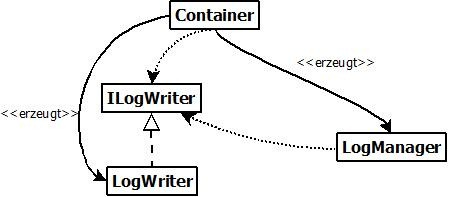
\includegraphics[width=9cm]{logging_looseCoupled.jpg}
\caption{Der Container erzeugt Instanzen und Injiziert Abhängigkeiten}
\end{figure}
\end{frame}

\begin{frame}
\frametitle{Kombination von Inversion Of Control mit Mocks}
\begin{itemize}
\item IoC - Vereinfachtes Einsetzen von Mocks und Stubs zur Testzeit und zentrale Verwaltung von Produktivkomponenten zur Produktivzeit
\item Mocks und Stubs - Ermöglicht die lose Kopplung von Programmkomponenten\\
Dadurch ermöglichen der testgetriebenen Entwicklung, da Programmkomponente als einzelnes testbar\\
\end{itemize}
\end{frame}

\section{Testgetriebene Entwicklung in der Praxis}
\begin{frame}
\frametitle{siehe Beispiel}
\end{frame}

\begin{appendix}
\begin{frame}
\frametitle{Quellen}
\begin{itemize}
\item http://www.codefest.at/post/2009/11/27/Design-Patterns-Teil-1-e28093-Inversion-of-Control-Dependency-Injection.aspx
\item http://www.code.google.com/p/mockito/
\item http://www.code.google.com/p/moq/
\item http://www.junit.sourceforge.net/javadoc/overview-summary.html
\item http://www.picocontainer.codehaus.org/
\item http://www.docs.structuremap.net/
\item http://www.webuser.hs-furtwangen.de/kaspar/seminar0607/TestDrivenDevelopement.pdf
\item OSHEROVE, Roy: the art of UNIT TESTING - with Examples in .NET. Manning Publications Co., 2009
\end{itemize}
\end{frame}
\end{appendix}

\end{document}